%%!TEX root = main.tex
\newcommand{\EvalHeight}{3.5cm}
\newcommand{\RndrHght}{3.2cm}
\newcommand{\RndrWdth}{4.1cm}
\newcommand{\CropWidth}{3.4cm}
\newcommand{\CropHght}{2.5cm}
\newcommand{\PanoWidth}{5.0cm}

\begin{figure*}
    \centering
    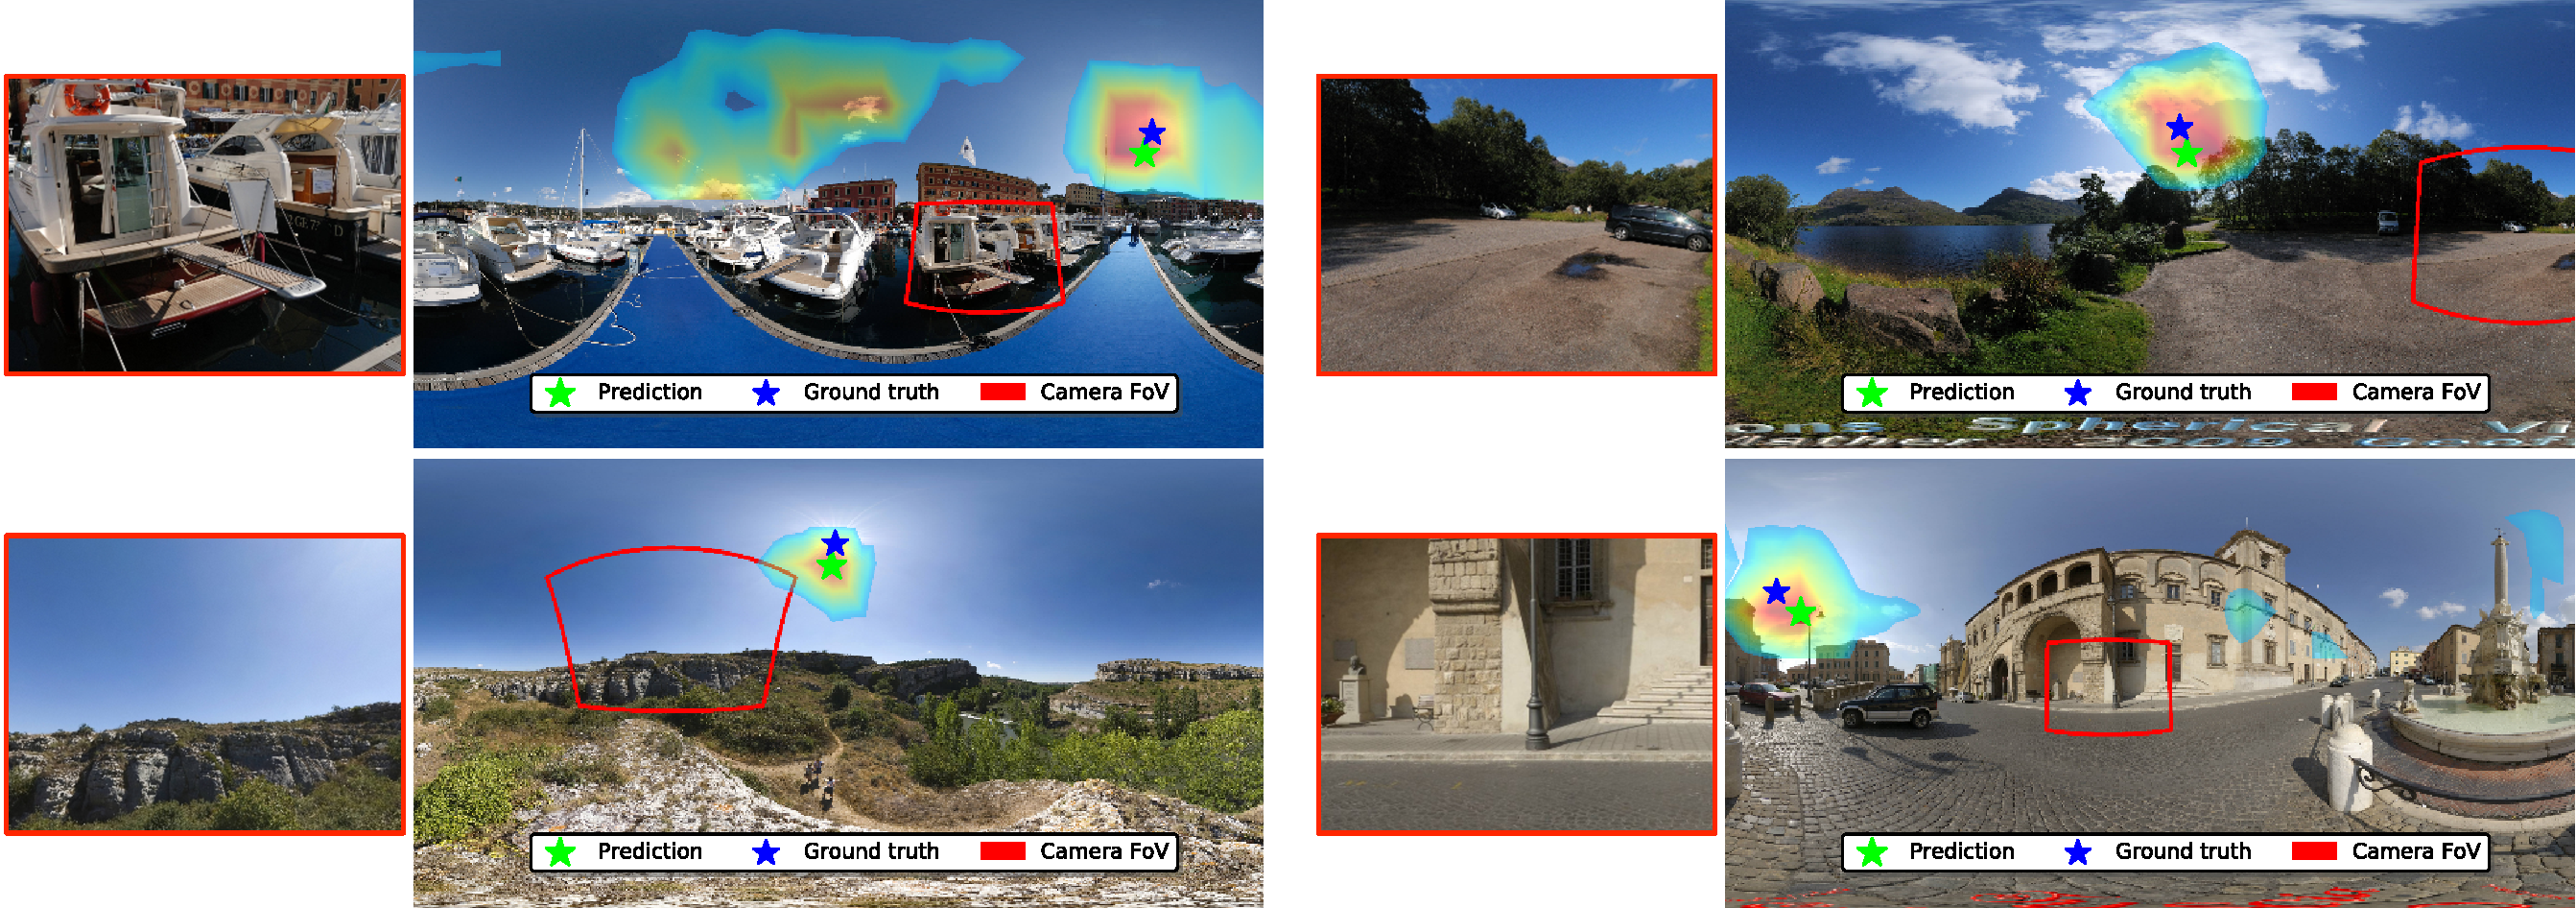
\includegraphics[width=\linewidth]{figures/sunpos_estim/sunpos.pdf}
%     \begin{tabular}{@{}cc@{}}
%   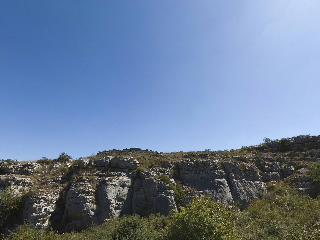
\includegraphics[width=\CropWidth,height=\CropHght]{./figures/sunpos_estim/crop/pano_aacuaoohjiliba_jpg-5.png}
% 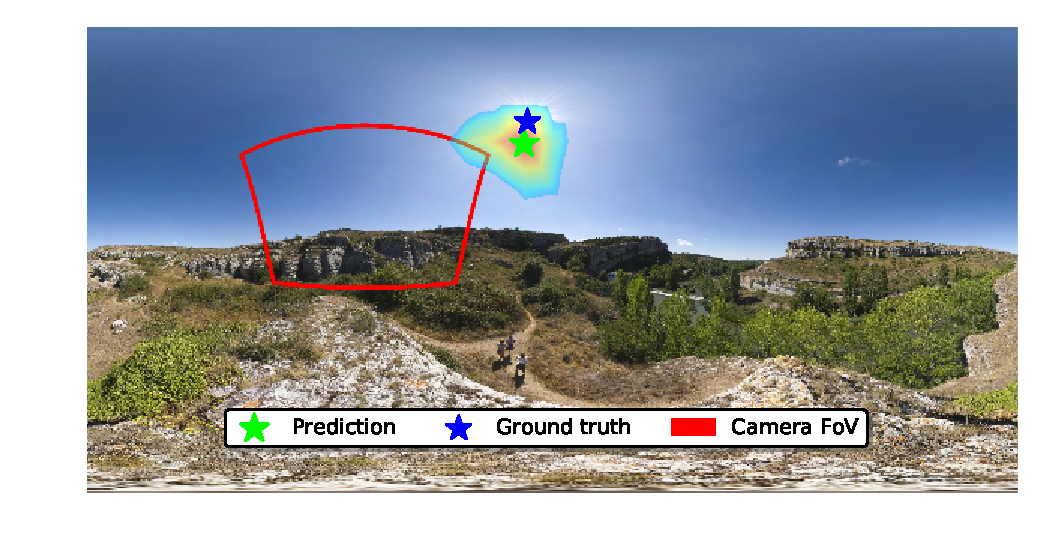
\includegraphics[width=\PanoWidth,height=\RndrHght,trim={1.1cm 1.1cm 0.1cm 0.4cm},clip]{./figures/sunpos_estim/panorama/pano_aacuaoohjiliba_jpg-5_png.pdf} &
%   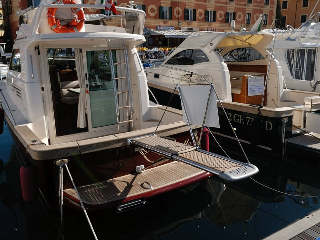
\includegraphics[width=\CropWidth,height=\CropHght]{./figures/sunpos_estim/crop/pano_aabljcacrurgxn_jpg-6.png}
% 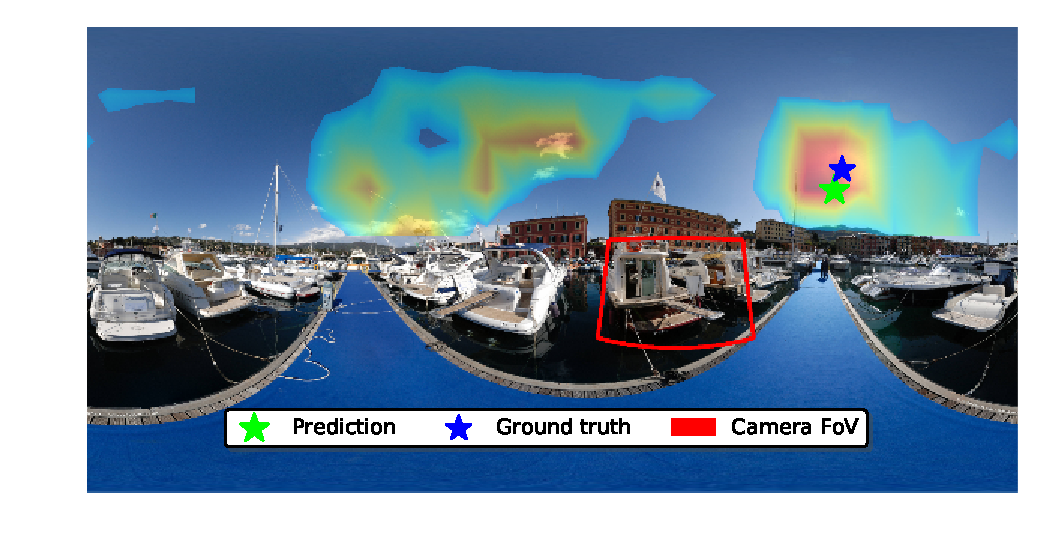
\includegraphics[width=\PanoWidth,height=\RndrHght,trim={1.1cm 1.1cm 0.1cm 0.4cm},clip]{./figures/sunpos_estim/panorama/pano_aabljcacrurgxn_jpg-6_png.pdf} \\
%   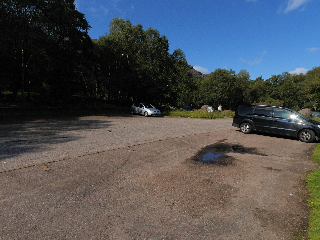
\includegraphics[width=\CropWidth,height=\CropHght]{./figures/sunpos_estim/crop/pano_aaihqlchfeptuj_jpg-1.png}
% 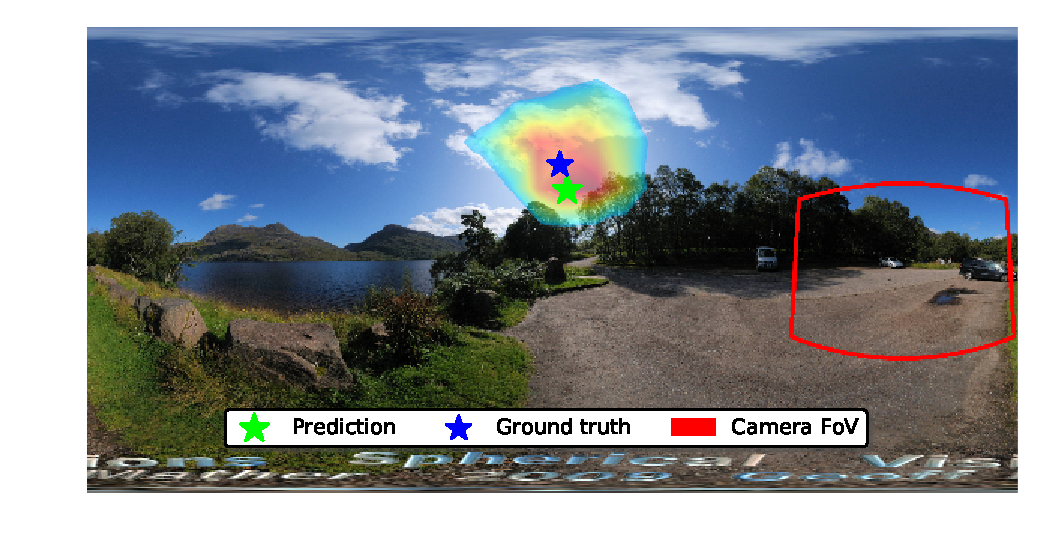
\includegraphics[width=\PanoWidth,height=\RndrHght,trim={1.1cm 1.1cm 0.1cm 0.4cm},clip]{./figures/sunpos_estim/panorama/pano_aaihqlchfeptuj_jpg-1_png.pdf} &
%   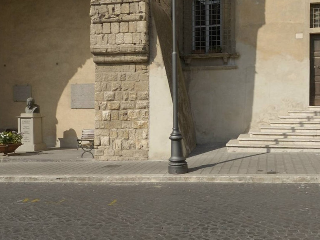
\includegraphics[width=\CropWidth,height=\CropHght]{./figures/sunpos_estim/crop/pano_aakpbaojeqowkb_jpg-3.png}
% 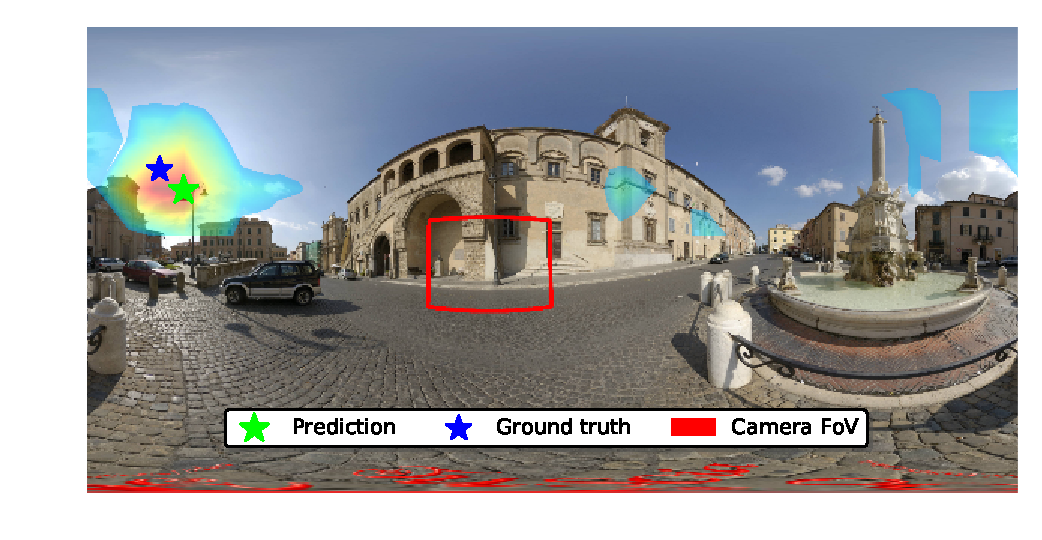
\includegraphics[width=\PanoWidth,height=\RndrHght,trim={1.1cm 1.1cm 0.1cm 0,4cm},clip]{./figures/sunpos_estim/panorama/pano_aakpbaojeqowkb_jpg-3_png.pdf}
    % \end{tabular}
    \caption[Examples of sun position estimation from a single outdoor image]{Examples of sun position estimation from a single outdoor image. For each example, the input image is shown on the left, and its corresponding location in the panorama is shown with a red outline. The color overlay displays the probability distribution of the sun position output by the neural network. A green star marks the most likely sun position estimated by the neural network, while a blue star marks the ground truth position. }
    \label{fig:evaluation_example_sun_position}
\end{figure*}

\section{Evaluation}
\label{sec:evaluation}

We evaluate the performance of the CNN at predicting the HDR sky environment map from a single image in a variety of ways. First, we present how well the network does at estimating the illumination parameters on the SUN360 dataset. We then show how virtual objects relit by the \emph{estimated} environment maps differ from their renders obtained with the ground truth parametric model, still on the SUN360. Finally, we acquired a small set of HDR outdoor panoramas, and compare our relighting results with those obtained with actual HDR environment maps. 

\subsection{Illumination parameters on SUN360}

\paragraph{Sun position}

We begin by evaluating the performance of the CNN at predicting the sun position from a single input image. Fig.~\ref{fig:evaluation_performance_sun_position} shows the quantitative performance at this task using three plots: the cumulative distribution function of sun angular estimation error, and detailed error histograms for each of the elevation and azimuth independently. We observe that 80\% of the test images have error less than 45\degree. Fig.~\ref{fig:evaluation_performance_sun_position}-(b) indicates that the network tends to underestimate the sun elevation in high elevation cases. This may be attributable to a lack of such occurrences in the training dataset---high sun elevations only occur between the tropics, and at specific times of year because of the Earth's tilted rotation axis. Fig.~\ref{fig:evaluation_performance_sun_position}-(c) shows that the CNN is not biased towards an azimuth position, and is robust across the entire range. Fig.~\ref{fig:evaluation_example_sun_position} shows examples of our sun position predictions overlayed over the panoramas that the test images were cropped from. Note that our method is able to accurately predict the sun direction across a wide range of scenes, field of views, and layouts.

We quantitatively compare our approach to that of \cite{lalonde-ijcv-12} at the task of sun azimuth estimation from a single image. Results are reported in fig.~\ref{fig:comparison-lalonde12}. First, fig.~\ref{fig:comparison-lalonde12}-(a) shows a comparison of both approaches on the 239-image dataset of \cite{lalonde-ijcv-12}. While our method has similar error in an octant (less than 22.5\degree), the precision in a quadrant (less than 45\degree) is significantly improved (by approximately 10\%) by our CNN-based approach. Fig.~\ref{fig:comparison-lalonde12}-(b) shows the same comparison on a 176-image subset of the SUN360 test set used in this chapter. In this case, the approach of Lalonde et al.~\cite{lalonde-ijcv-12} fails while the CNN reports robust performance, comparable to fig.~\ref{fig:comparison-lalonde12}-(a). This is probably due to the fact that the SUN360 test set contains much more challenging images that are often devoid of strong, explicit illumination cues. These cues, which are expressly relied upon by \cite{lalonde-ijcv-12}, are critical to the success of such methods.
%In contrast, our CNN is robust to their absence, yet is still able to extract useful illumination information from the images. 
\vspace{-1.5em}
\paragraph{Turbidity and exposure}

\begin{figure}[!th]
    \centering
    \footnotesize
    \setlength{\tabcolsep}{1pt}
    \begin{tabular}{cc}
    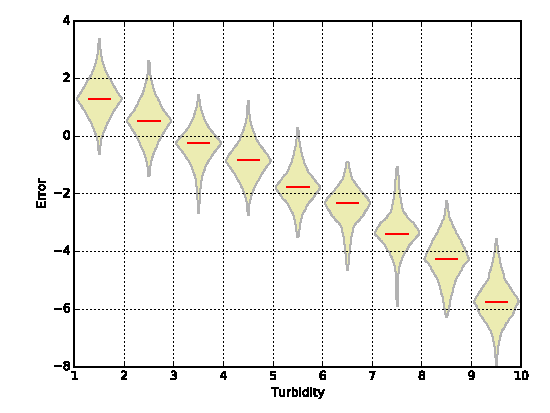
\includegraphics[height=5cm]{figures/evaluation_performances/dist-turdibity.pdf} &
    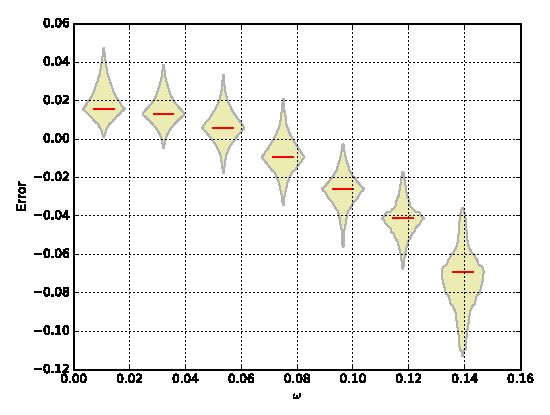
\includegraphics[height=5cm]{./figures/evaluation_performances/dist-omega.pdf} \\
    (a) Turbidity $t$ &
    (b) Exposure $\omega$ 
    \end{tabular}
    \vspace{.25em}
    \caption[Quantitative evaluation for turbidity $t$ and exposure $\omega$]{Quantitative evaluation for turbidity $t$ and exposure $\omega$. The distribution of errors are displayed as ``box-percentile'' plots (see fig.~\ref{fig:evaluation_performance_sun_position}). The CNN tends to favor clear skies (low turbidity), and has higher errors when the exposure is high.}
    \label{fig:evaluation_sky_parameters}
\end{figure}

\begin{figure}[!t]
\centering
\footnotesize
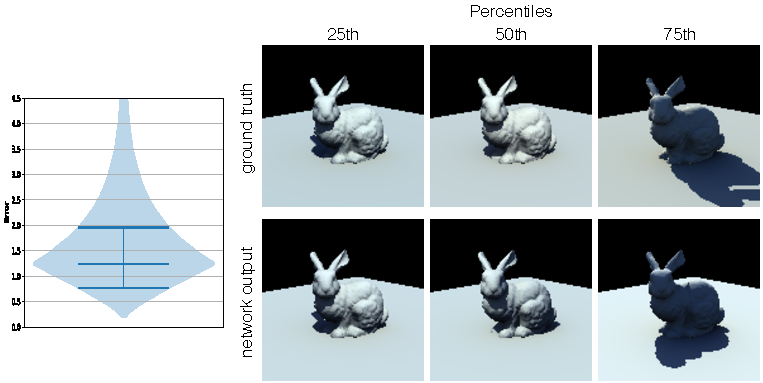
\includegraphics[width=0.6\linewidth]{figures/validation-sun360/rmse-horiz.pdf} \\
(a) RMSE \\
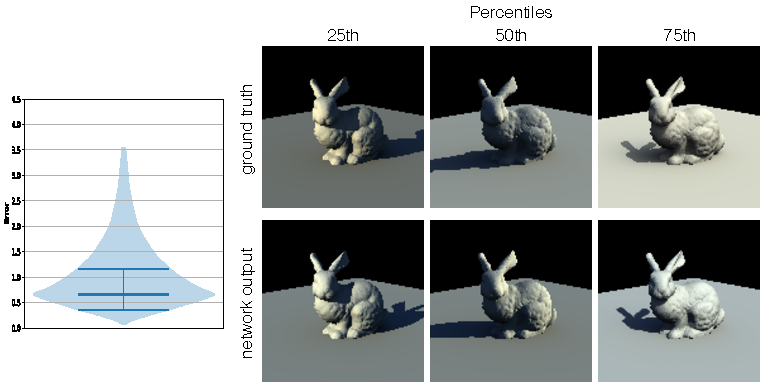
\includegraphics[width=0.6\linewidth]{figures/validation-sun360/rmse-si-horiz.pdf} \\
(b) Scale-invariant RMSE \\
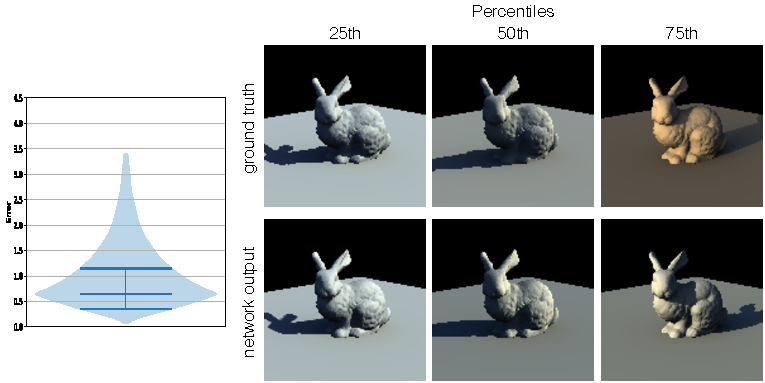
\includegraphics[width=0.6\linewidth]{figures/validation-sun360/rmse-si-rgb-horiz.pdf} \\
(c) Per-color scale-invariant RMSE \\
\vspace{.25em}
\caption[Quantitative relighting comparison with ground truth lighting on SUN360]{Quantitative relighting comparison with the ground truth lighting parameters on the SUN360 dataset. We compute three types of error metrics: (a) RMSE, (b) scale-invariant RMSE~\cite{grosse-iccv-09}, and (c) per-color scale-invariant RMSE. The plots on the left shows the distribution of errors with the median, 25th and 75th percentiles identified with blue bars. For each measure, examples corresponding to particular error levels are shown to give a qualitative sense of performance. Renders obtained with the ground truth (estimated) lighting parameters are shown in the top (bottom) row.}
\label{fig:quantitative-relighting-sun360}
\vspace{-1em}
\end{figure}

% \begin{figure}[!th]
% 	\centering
%     \footnotesize
%     \setlength{\tabcolsep}{1pt}
%     \begin{tabular}{cc}
%     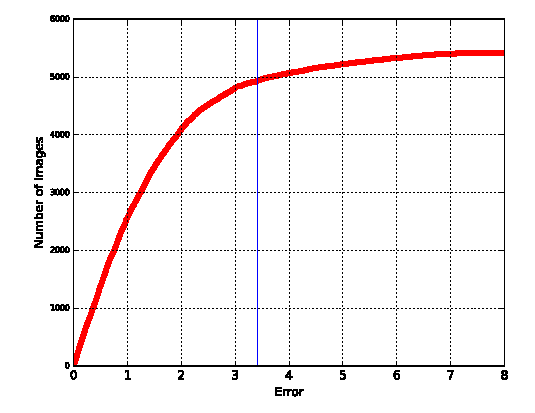
\includegraphics[height=3.1cm]{./figures/evaluation_performances/cdf-turbidity.pdf} & 
%     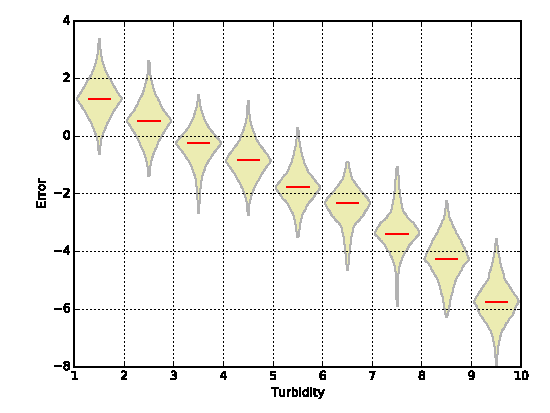
\includegraphics[height=3.1cm]{figures/evaluation_performances/dist-turdibity.pdf} \\
%     \multicolumn{2}{c}{(a) Turbidity $t$} \\
%     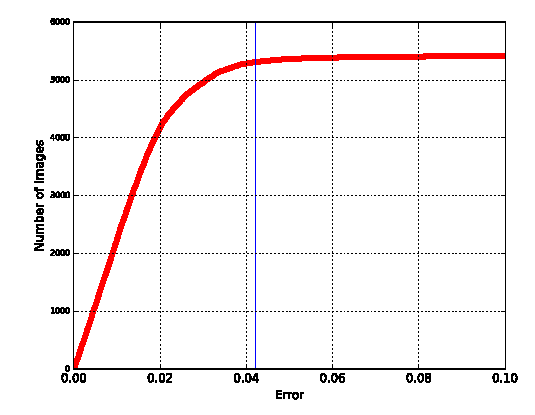
\includegraphics[height=3.1cm]{./figures/evaluation_performances/cdf-omega.pdf} &
%     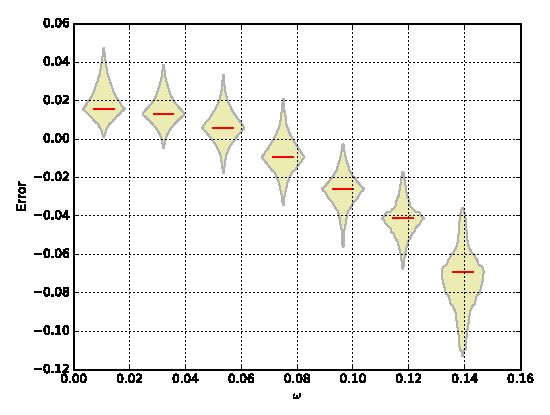
\includegraphics[height=3.1cm]{./figures/evaluation_performances/dist-omega.pdf} \\
%     \multicolumn{2}{c}{(b) Exposure $\omega$}
%     \end{tabular}
%     \vspace{.5em}
% 	\caption{Quantitative evaluation for turbidity $t$ and exposure $\omega$. Estimation error on turbidity $t$ as (a) a cumulative distribution function (CDF) of errors and (b) a ``box-percentile plot'' (see fig.~\ref{fig:evaluation_performance_sun_position}). We recover a turbidity within 2 units for 75\% of the test images. The CNN tends to favor clear skies (low turbidity). Estimation error on exposure $\omega$ as (a) the CDF of errors and (b) a ``box-percentile plot''. In this case, the network has higher errors when the exposure is high.}
% 	\label{fig:evaluation_sky_parameters}
% \end{figure}

We evaluate the regression performance for the turbidity $t$ and exposure $\omega$ lighting parameters on the SUN360 test set, and report the results in fig.~\ref{fig:evaluation_sky_parameters}. Overall, the network tends to favor low turbidity estimates of the sky (as the dataset contains a majority of such examples). In addition, the network successfully estimates low exposure values, but has a tendency to underestimate images with high exposures.%, likely resulting in renders which are too dark. 
\vspace{-1.5em}
\paragraph{Camera parameters}

A detailed performance analysis is available in the supplementary material. In a nutshell, the CNN achieves error of less than 7\degree ~for the elevation and 11\degree ~in field of view for 80\% of the test images. 

% \subsubsection{Camera parameters}

% \begin{figure*}[!ht]
% 	\centering
%     \footnotesize
%     \begin{tabular}{c@{}c@{}c@{}c}
%     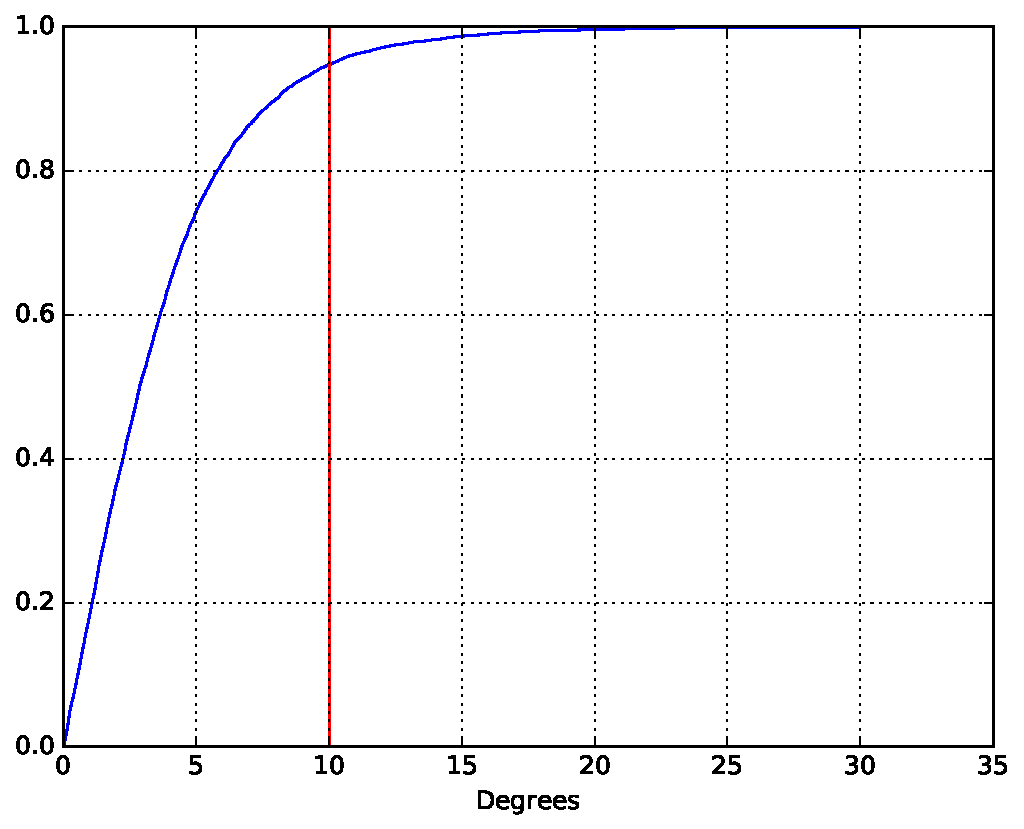
\includegraphics[width=0.247\linewidth,height=\EvalHeight]{./figures/evaluation_performances/cdf_2.pdf} &
%     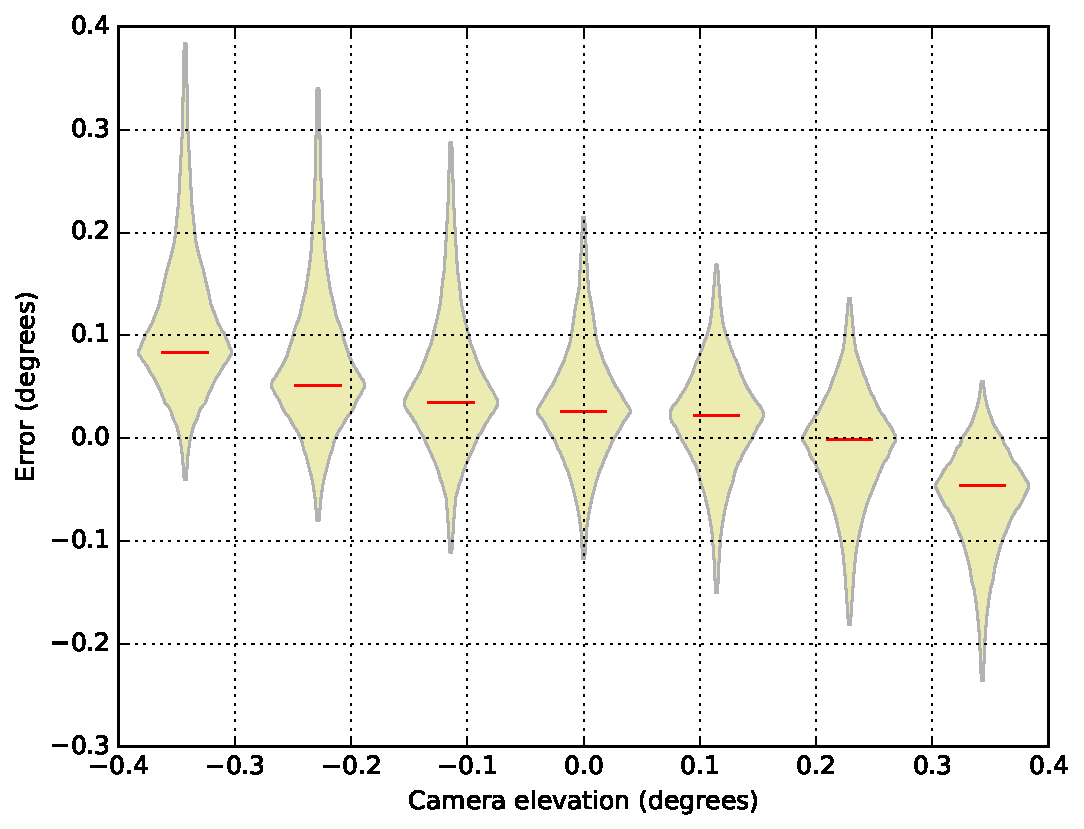
\includegraphics[width=0.247\linewidth,height=\EvalHeight]{./figures/evaluation_performances/box-percentile_plot_2.pdf} &
%    	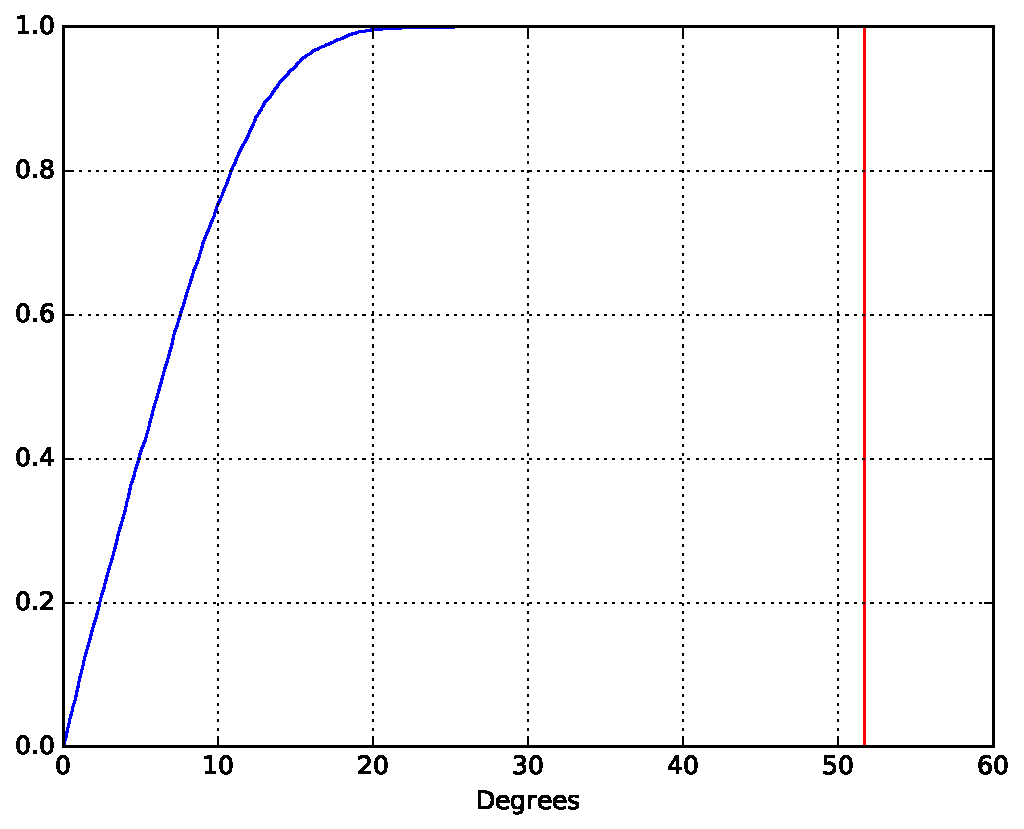
\includegraphics[width=0.247\linewidth,height=\EvalHeight]{./figures/evaluation_performances/cdf_3.pdf} &
%    	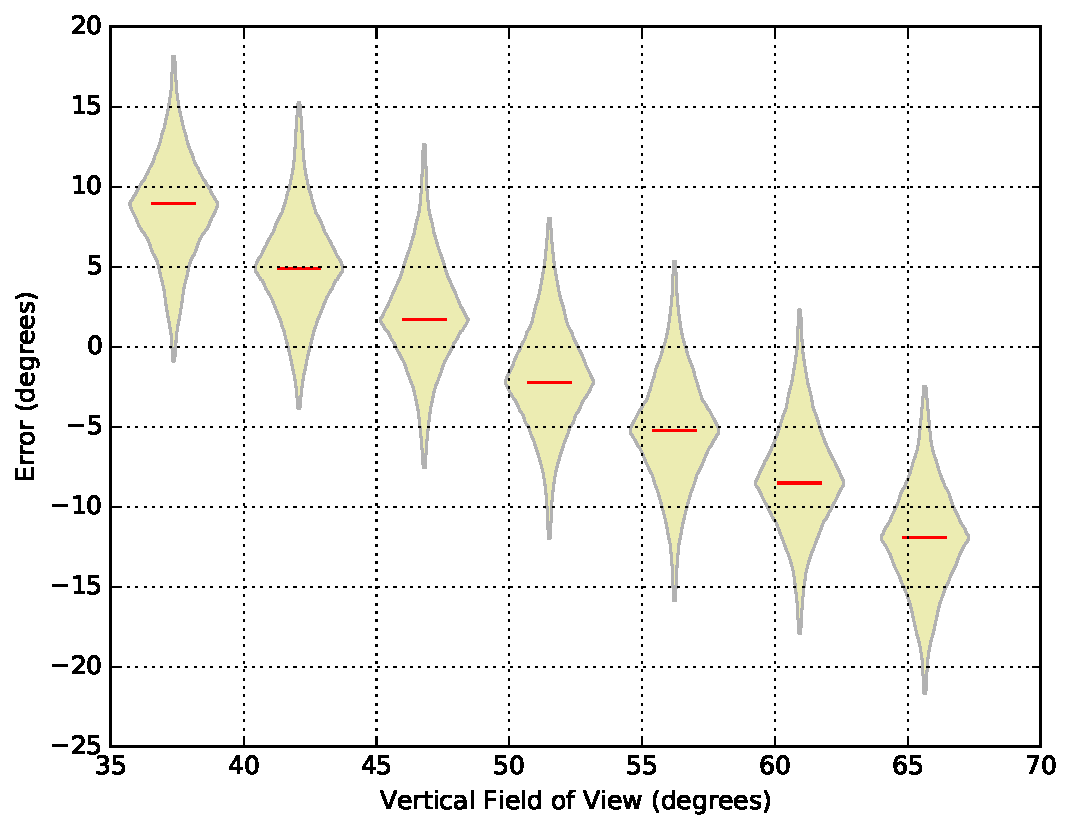
\includegraphics[width=0.247\linewidth,height=\EvalHeight]{./figures/evaluation_performances/box-percentile_plot_3.pdf} \\
%     (a) Camera elevation & (b) Camera elevation & (c) Field of view & (d) Field of view
%     \end{tabular}
% 	\caption{Estimation error on camera parameters: elevation (horizon estimation) (a), (b) and field of view (c), (d).}
% 	\label{fig:evaluation_camera_parameters}
% \end{figure*}

% Show error in horizon estimation (camera elevation) and viewing field of view.

\begin{figure}[!th]
    \centering
    \footnotesize
    \setlength{\tabcolsep}{1pt}
    \begin{tabular}{cc}
    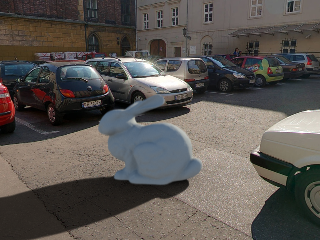
\includegraphics[width=.47\linewidth]{./figures/renders/netout/pano_aaafspbtffjzbn_jpg-1_png_out.png} &
    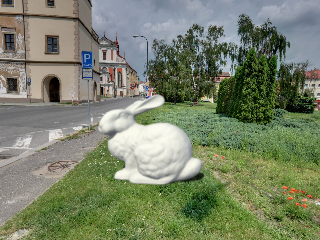
\includegraphics[width=.47\linewidth]{./figures/renders/netout/pano_abauwcbvavypmw_jpg-2_png_out.png} \\
    % 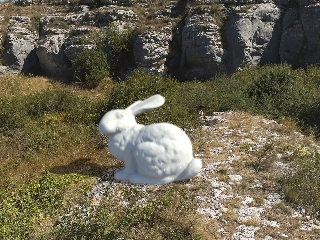
\includegraphics[width=.47\linewidth]{./figures/renders/netout/pano_aacuaoohjiliba_jpg-4_png_out.png} &
    % 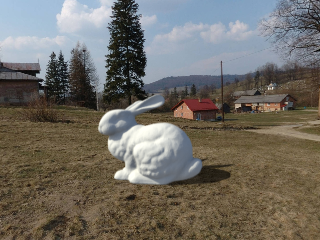
\includegraphics[width=.47\linewidth]{./figures/renders/netout/pano_akvgrwlvpakobh_jpg-6_png_out.png} \\
    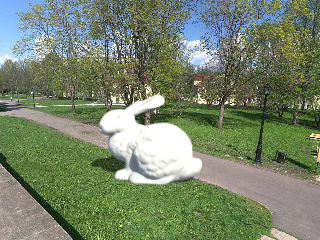
\includegraphics[width=.47\linewidth]{./figures/renders/netout/pano_ajmdcorvpbtdcb_jpg-3_png_out.png} &
    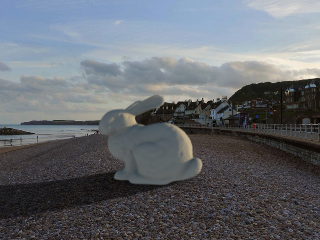
\includegraphics[width=.47\linewidth]{./figures/renders/netout/pano_ajwnburtukssxf_jpg-5_png_out.png}
    \end{tabular}
    \caption[Virtual object insertion with authomated lighting estimation]{Virtual object insertion with automated lighting estimation. From a single image, the CNN predicted a full HDR sky map, which is used to render an object into the image. No additional steps are required. More results on automated object insertion are available in the supplementary materials.}
    \label{fig:evaluation_render_examples}
\end{figure}

\begin{figure}[!th]
    \centering
    \footnotesize
    \setlength{\tabcolsep}{1pt}
    \begin{tabular}{ccc}
    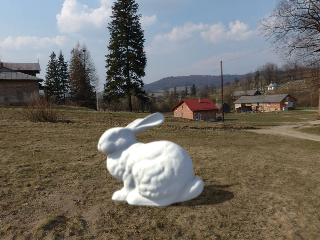
\includegraphics[width=.47\linewidth]{figures/renders/elevation/pano_akvgrwlvpakobh_jpg-6_png_out.png} & 
    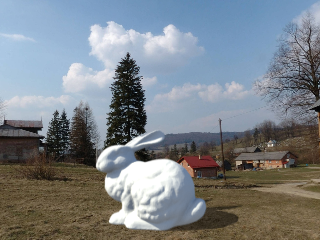
\includegraphics[width=.47\linewidth]{figures/renders/elevation/pano_akvgrwlvpakobh_jpg-6_png_out_tilted.png} \\
    Estimated elevation: -9\degree & 
    Estimated elevation: 3.5\degree & 
    \end{tabular}
    \vspace{.25em}
    \caption[Virtual object insertion with automated lighting and camera elevation estimation]{Virtual object insertion with automated lighting and camera elevation estimation. The two images are taken at the same location with the camera pointing downwards (left) and upwards (right). The elevation of the virtual camera used to render the bunny model is set to the value predicted by the CNN, resulting in a bunny which realistically rests on the ground.}
    \label{fig:evaluation-elevation}
    \vspace{-1em}
\end{figure}

\subsection{Relighting on SUN360}

Another way of evaluating the performance is by comparing the appearance of a Lambertian 3D model rendered with the estimated lighting, with that of the same model lit by the ground truth. Fig.~\ref{fig:quantitative-relighting-sun360} provides such a comparison, by showing three different error metrics computed on renderings obtained on our test set. The error metrics are the (a) RMSE, (b) scale-invariant RMSE, and (c) per-color scale-invariant RMSE. The scale-invariant versions of RMSE are defined similarly to Grosse et al.~\cite{grosse-iccv-09}, except that the scale factor is computed on the entire image (instead of locally as in~\cite{grosse-iccv-09}). The ``per-color'' variant computes a different scale factor for each color channel to mitigate differences in white balance. The black background in the renders is masked out before computing the metrics.
  
To give a sense of what those numbers mean qualitatively, fig.~\ref{fig:quantitative-relighting-sun360} also provides examples corresponding to each of the (25, 50, 75)th error percentiles. Even examples in the 75th error percentile look good qualitatively. Slight differences in the sun direction and the overall color can be observed, but they still lie within reasonable limits.

Fig.~\ref{fig:evaluation_render_examples} shows examples of virtual objects inserted into images after being rendered with our estimated HDR illumination. As these examples show, our technique is able to infer plausible illumination conditions ranging from sunny to overcast, and high noon to dawn/dusk, resulting in natural-looking composite images. Fig.~\ref{fig:evaluation-elevation} shows that the camera elevation estimated from the CNN can be used within the rendering pipeline to automatically rotate the virtual camera used to render the object. In these results, a simple ground plane is used to model the interactions between the virtual object and its environment, and the object is placed manually at a fixed distance in front of the camera.


\begin{figure*}[t]
    \centering 
    \footnotesize
    \setlength{\tabcolsep}{1pt}
    \begin{tabular}{cccccc}
    Ground truth & Estimated & Ground truth & Estimated & Ground truth & Estimated \\
    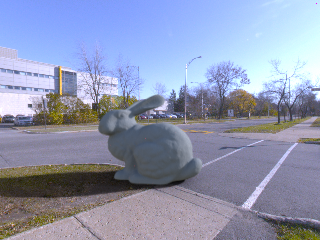
\includegraphics[width=.16\linewidth]{./figures/valid/gt/AG8A2749_Panorama_hdr-corrected_exr-0_png_out.png} &
    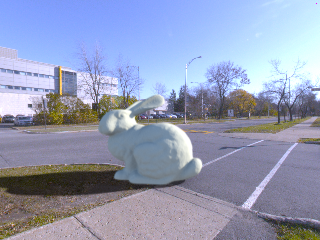
\includegraphics[width=.16\linewidth]{./figures/valid/cnn/AG8A2749_Panorama_hdr-corrected_exr-0_png_out.png}\: &
    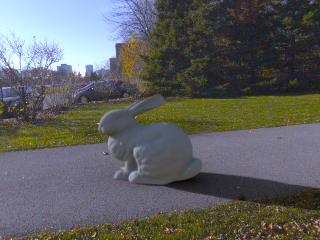
\includegraphics[width=.16\linewidth]{./figures/valid/gt/AG8A2791_Panorama_hdr-corrected_exr-2_png_out.png} &
    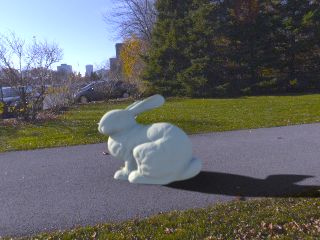
\includegraphics[width=.16\linewidth]{./figures/valid/cnn/AG8A2791_Panorama_hdr-corrected_exr-2_png_out.png}\: &
    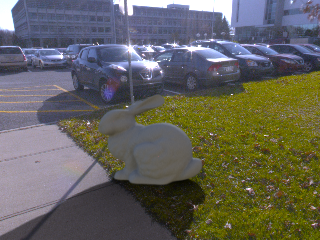
\includegraphics[width=.16\linewidth]{./figures/valid/gt/AG8A3169_Panorama_hdr-corrected_exr-5_png_out.png} &
    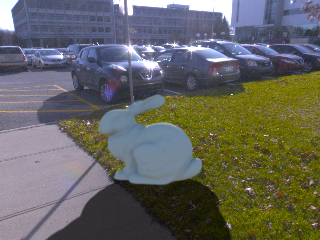
\includegraphics[width=.16\linewidth]{./figures/valid/cnn/AG8A3169_Panorama_hdr-corrected_exr-5_png_out.png} \\
    \multicolumn{2}{c}{
    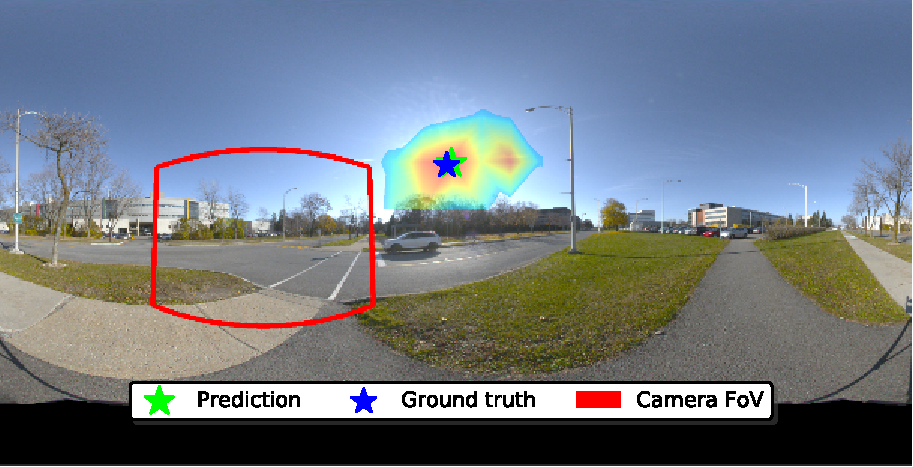
\includegraphics[width=\RndrWdth]{./figures/valid/panos/AG8A2749_Panorama_hdr-corrected_exr-0_png.pdf}} &
    \multicolumn{2}{c}{
    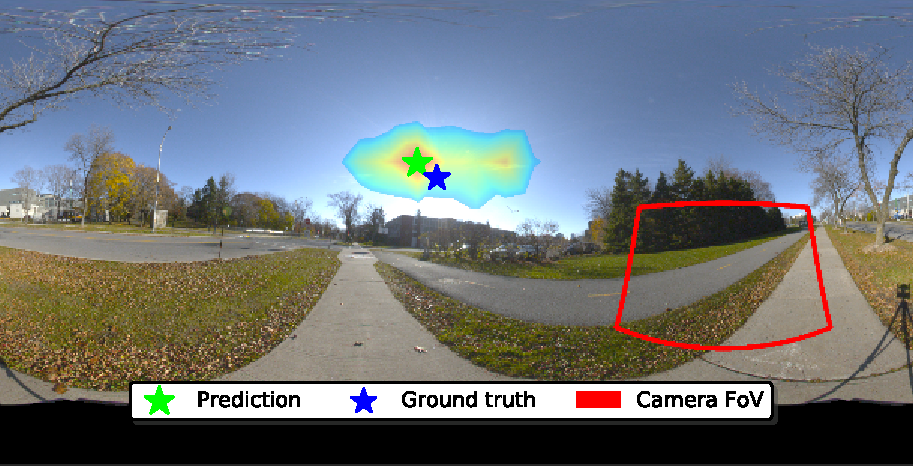
\includegraphics[width=\RndrWdth]{./figures/valid/panos/AG8A2791_Panorama_hdr-corrected_exr-3_png.pdf}} &
    \multicolumn{2}{c}{
    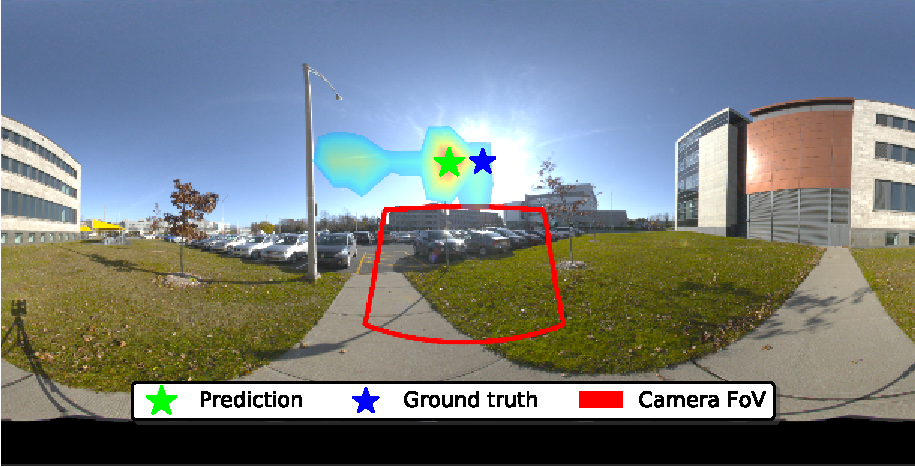
\includegraphics[width=\RndrWdth]{./figures/valid/panos/AG8A3169_Panorama_hdr-corrected_exr-5_png.pdf}} \\
    \multicolumn{2}{c}{(a)} & \multicolumn{2}{c}{(b)} & \multicolumn{2}{c}{(c)}
    \end{tabular}
    \caption[Object relighting comparison with ground truth illumination conditions on HDR panoramas]{Object relighting comparison with ground truth illumination conditions on captured HDR panoramas. For each example, the top row shows (left) a bunny model relit by the ground truth HDR illumination conditions captured in situ; (right) the same bunny model, relit by the illumination conditions estimated by the CNN solely from the background image, completely automatically. No further adjustment (e.g. overall brightness, saturation, etc.) was performed. The bottom row shows the original environment map, field of view of the camera (in red), and the distribution on sun position estimation (as in fig.~\ref{fig:evaluation_example_sun_position}). Please see additional results on our project page.}
    \label{fig:hdr-panoramas-validation}
    \vspace{-1em}
\end{figure*}

\subsection{Validation with HDR panoramas}
\label{subsec:relighting_hdr}

To further validate our approach, we captured a small dataset of 19 unsaturated, outdoor HDR panoramas. To properly expose the extreme dynamic range of outdoor lighting, we follow the approach proposed by Stumpfel et al.~\cite{stumpfel-afrigraph-04}. We captured 7 bracketed exposures ranging from 1/8000 to 8 seconds at f/16, using a Canon EOS 5D Mark III camera installed on a tripod, and fitted with a Sigma EXDG 8mm fisheye lens. A 3.0 ND filter was installed behind the lens, necessary to accurately measure the sun intensity. The exposures were stored as 14-bit RAW images at full resolution. The process was repeated at 6 azimuth angles by increments of 60\degree ~to cover the entire 360\degree ~panorama. The resulting 42 images were fused using the \textsc{PTGui} commercial stitching software. To facilitate the capture process, the camera was mounted on a programmable robotic tripod head, allowing for repeatable and precise capture. % Fig.~\ref{fig:hdr-panoramas} shows an example of such an HDR panorama captured using this method. 

% \begin{figure}[!th]
% \centering
% \footnotesize
% 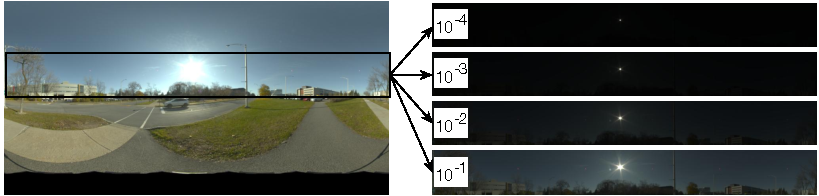
\includegraphics[width=\linewidth]{figures/smalldb/db-sunny.pdf}
% \caption{Example HDR panorama captured with the robotic tripod head. The outlined region on the left is shown at four different exposures on the right (from $10^{-1}$ to $10^{-4}$) to highlight that the extremely high dynamic range of outdoor lighting is properly captured (please zoom in the electronic version).}
% \label{fig:hdr-panoramas}
% \end{figure}

To validate the approach, we extract limited field of view photos from the HDR panoramas and save them as JPEG files. The CNN is then applied to the input photos to predict their illumination conditions. Then, we compare relighting results obtained by rendering a bunny model with: 1) the HDR panorama itself, which represents the ground truth lighting conditions; and 2) the estimated lighting conditions. Example results are shown in fig.~\ref{fig:hdr-panoramas-validation}. While we note that the exposure $\omega$ is slightly overestimated (resulting in a render that is brighter than the ground truth), the relit bunny appears quite realistic. 
% \KS{comparison of predicted illumination parameters vs fits? How much of the error is from the fit?}
  
\begin{figure}
    \centering
    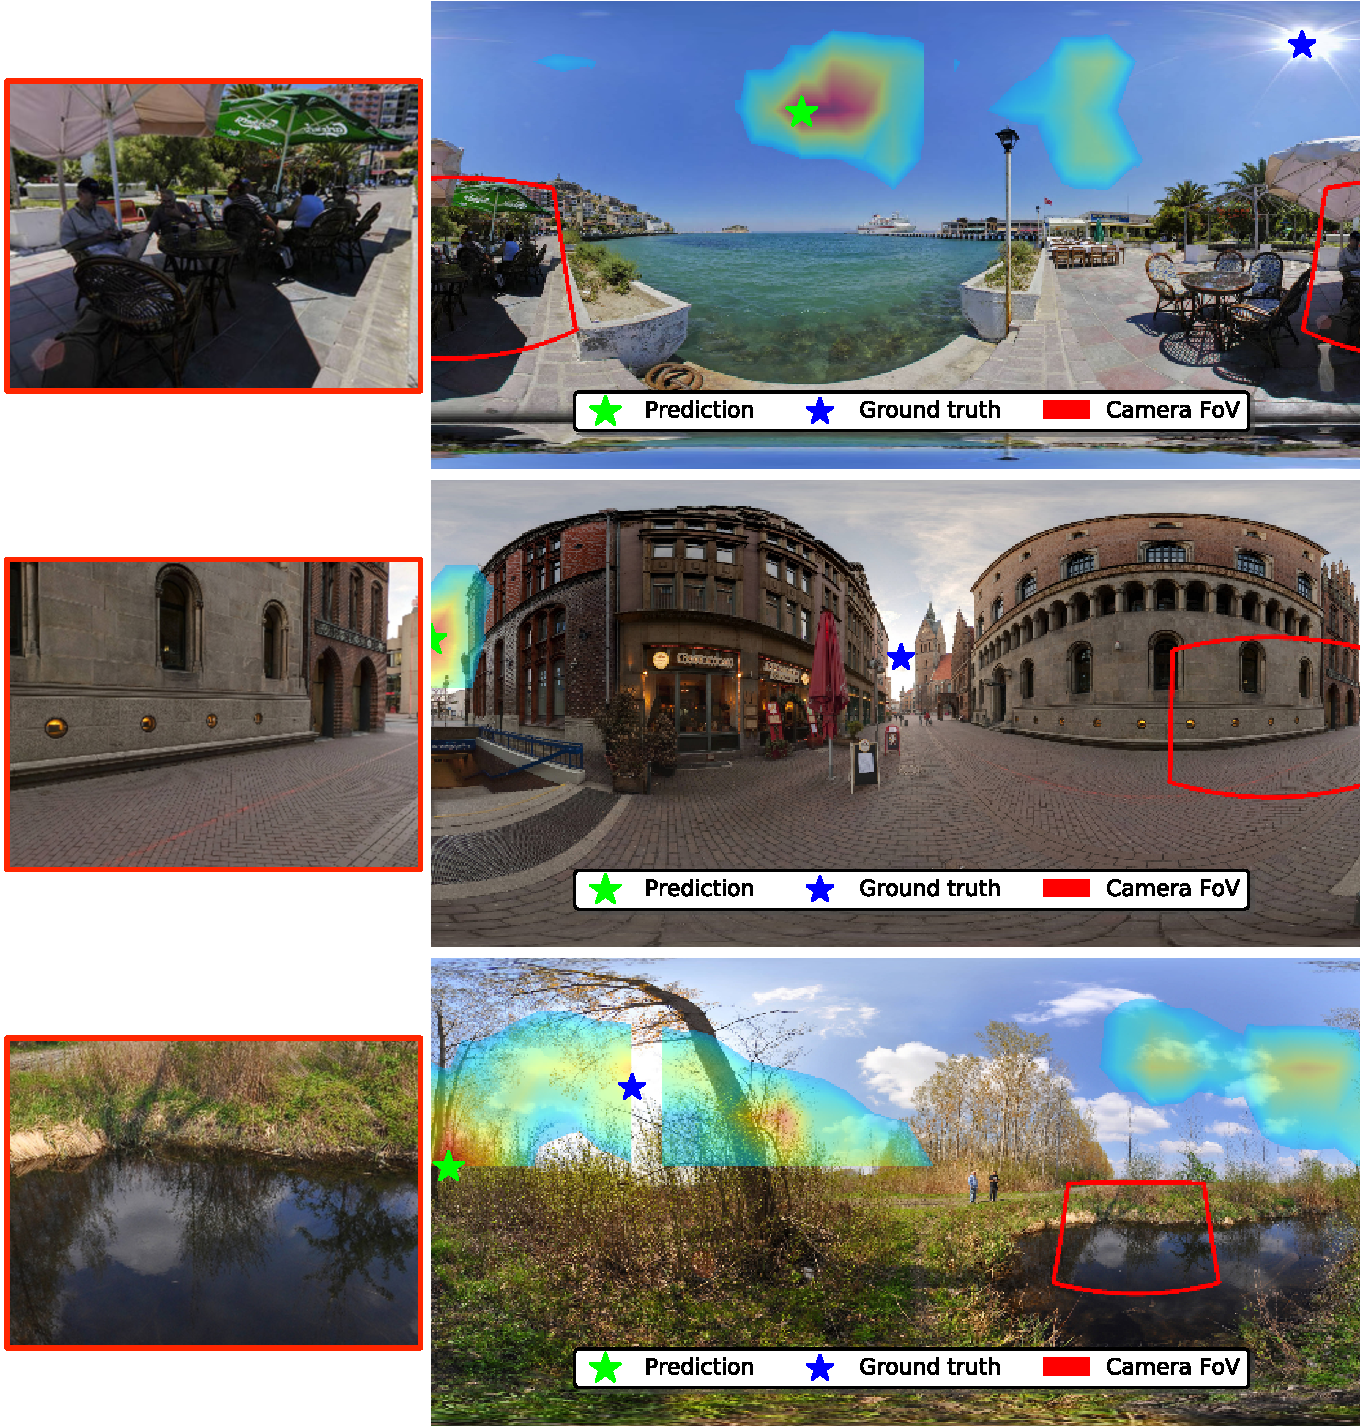
\includegraphics[width=\linewidth]{figures/sunpos_estim_failure/sunpos_failure_cases.pdf}
    \caption[Typical failure cases of sun position estimation]{Typical failure cases of sun position estimation from a single outdoor image. See fig.~\ref{fig:evaluation_example_sun_position} for an explanation of the annotations. Failure cases occur when illumination cues are mixed with complex geometry (top), absent from the image (middle), or in the presence of mirror-like surfaces (bottom).}
    \label{fig:evaluation_example_sun_position_failure_cases}
    %\vspace{-2em}
\end{figure}

